\subsection{$A_5^{\mathrm{1-loop}}[1^-2^-3^+4^+5^+]$ in $\mathcal{N}=4$ super Yang-Mills}
Let us see how to use quadruple cuts to extract box coefficients. 
There are four possible configurations for the external momenta under a quadruple cut.
Each of the configurations corresponds to a one-mass box integral.
Among the four tree-level amplitudes that we obtain from a quadruple cut~\cref{box_coeff}, there is a four-point amplitude and three three-point ones.
As already noted in~\cite{Britto:2004nc}, massless legs in quadruple cut would lead to inconsistent results if we choose loop-momentun to be real\footnote{This was handled in~\cite{Britto:2004nc} by working in the signature $(--++)$.}. 
However, in the contour integral scheme with complex loop momentum that we mentioned earlier, this problem is not present.
\\\\
Next, let us consider all the possible helicity configuration on the cuts.
To start, we may take all the internal particles to be gluons. 
Then, we relate the all-gluon tree-level amplitudes to other amplitudes with different species by~\cref{super_wi}. 
By the discussion given in section~\ref{sect-spinor}, we have to have exactly two particles of the same helicity in order to get non-vanishing contribution from three- and four-point tree-level amplitudes.
Up to this step, we have already eliminate a bunch of helicity configurations
\\\\
Finally, the on-shell condition of the internal propagtors may in certain case impose further relationships to the external momenta than just the momentum conservation.
These cases should also be discarded because they violate our requirement of non-collinearity of the external momenta. 
\color{red}perhaps describe more with a graph.\color{black}
At the end of the day, there are only five possible solution to the all-gluon configuration.
We give the detailed computation hereunder.
\\\\
\begin{figure}[h]
  \centering
  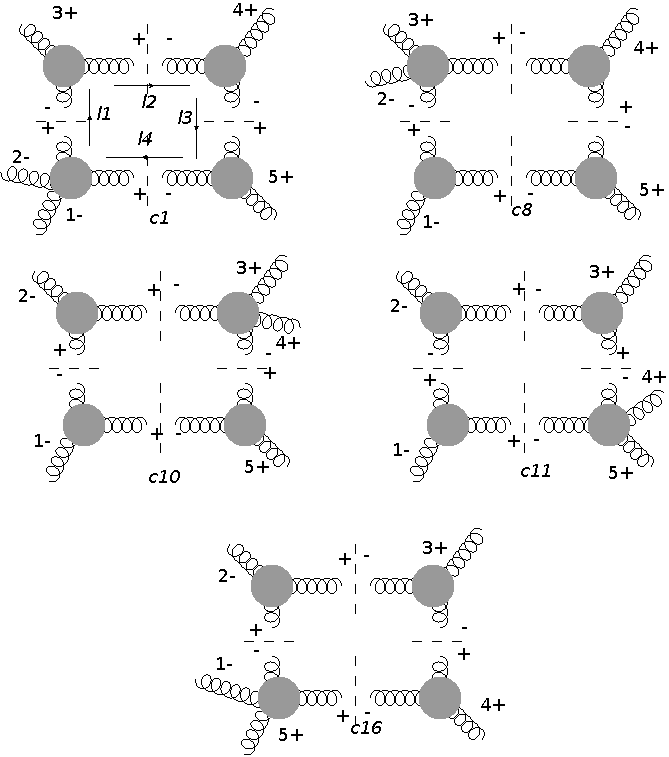
\includegraphics[width=0.8\linewidth]{A5mhv.png}
  \caption{The only non-vanishing contributions for $A_5^{\mathrm{1-loop}}[1^-2^-3^+4^+5^+]$ in $\mathcal{N}=4$ super Yang-Mills}
  \label{fig-cutkosky}
\end{figure}
\paragraph{\ref{A5-1}}
The special three-particle kinematics tells us that either the square spinor product or the angle one of any two on-shell spinor linked with a trivalent vertex vanishes.
By considering the trivalent vertices appearing in the cut~\cref{A5-1}, the only possible solution for the internal momenta in terms should satisfy
\begin{equation*}
|l_1\rangle = \alpha |5\rangle \quad,\quad
|l_2\rangle = \delta |3\rangle \quad,\quad
|l_3\rangle = \gamma |l_3\rangle\quad,\quad
|l_3] = \eta|4]\quad,\quad
|l_4] = \beta 4]
\end{equation*}
Hence, the coefficient determined by~\cref{box_coeff} is
\begin{equation*}
\begin{split}
c_1 = &
\frac{1}{2}\frac{\langle 12 \rangle^4}{\langle 1 2 \rangle \langle 2 l_2\rangle \langle l_2 l_1 \rangle\langle l_1 1 \rangle}
\frac{[3l_3]^3}{[l_3 l_2][l_2 3]}
\frac{\langle l_3 l_4 \rangle^{3}}{\langle l_4 4 \rangle \langle 4 l_3\rangle}
\frac{[l_4 5 ]^3}{[5l_1][l_1 l_4]}
\\
= & 
\frac{1}{2}\frac{\langle 12 \rangle^3}{\langle 2 l_2 \rangle\langle l_2 l_1 \rangle\langle l_1 1\rangle}
\frac{[34]^2\langle l_4 4\rangle}{[l_3 l_2][l_2 3]\langle 4 l_3\rangle}
\frac{[l_4 5]^2}{[5l_1 ][l_1 l_4]}
[3 l_3]\langle l_3 l_4 \rangle [l_4 5]
\\
= &
\frac{1}{2}
\frac{\langle 12 \rangle^3[34]^2[45]}{\langle 15 \rangle\langle2|\slashed{K}_{3}|4]}
\\
= &
\frac{1}{2}\frac{\langle 12 \rangle^4 s_{34}s_{45}}{\langle 12 \rangle\langle 23 \rangle \langle 34\rangle \langle 45\rangle \langle 51\rangle}
\\
= &
\frac{1}{2}s_{34}s_{45}A_5^{\textrm{MHV-tree}}[12345]
\end{split}
\end{equation*}
As we will see, all the contributions that we will compute are related to the tree-level amplitude by the same structure as given in the last line.   
%
%
%%%%%%%%%%%%%
%
\iffalse
\begin{figure}
  \centering
    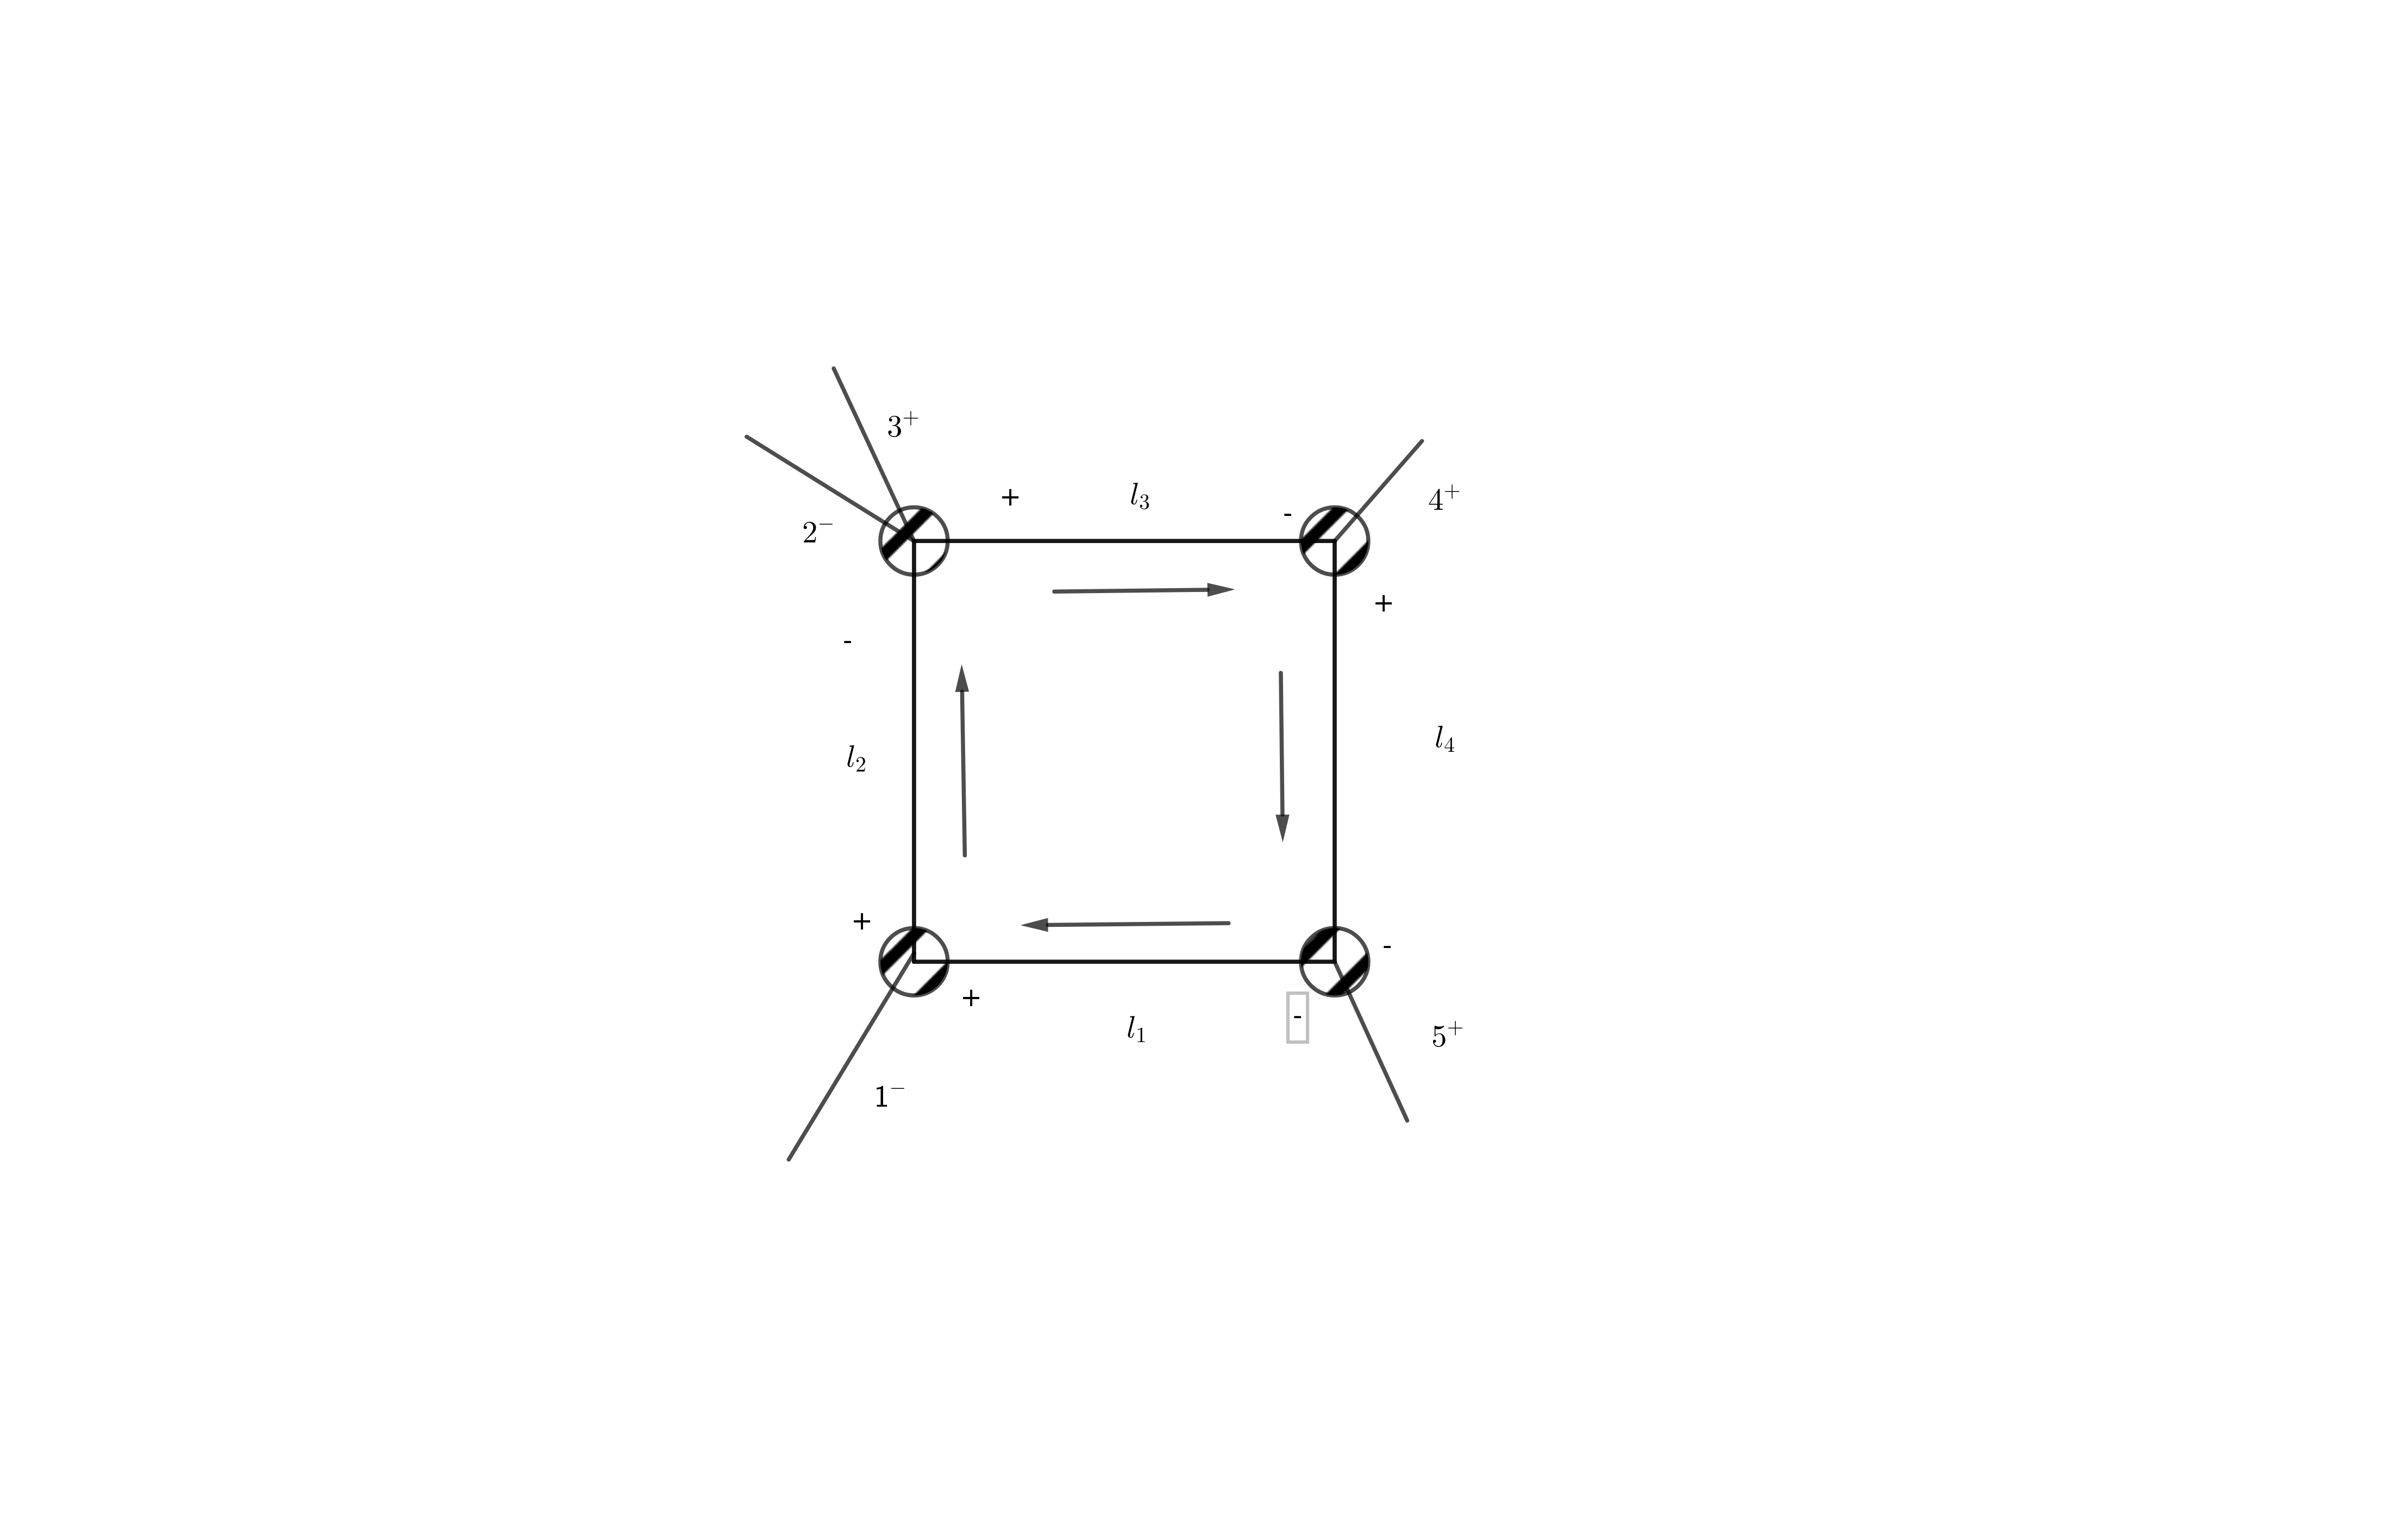
\includegraphics[width=\linewidth]{A5-8}
    \caption{A5-8}
  \label{A5-8}
\end{figure}
\fi
\paragraph{\ref{A5-8}}
By~\cref{box_coeff}, the box coefficient corresponding to this contribution is
\begin{equation*}
\begin{split}
c_8 = & \frac{1}{2}
\frac{[l_1 l_2]^3}{[l_1 1][1l_2]}
\frac{\langle 2 l_2 \rangle^4}{\langle 2l_2 \rangle\langle l_2 l_3\rangle\langle l_3 3 \rangle\langle 32 \rangle}
\frac{[l_4 4 ]^3}{[l_4 l_3][l_3 4]}
\frac{\langle l_4 l_1 \rangle^3}{\langle l_4 5 \rangle\langle 5 l_1\rangle}
\\
= &
\frac{\langle 12 \rangle^3[1l_1 ]\langle l_1 5\rangle^2 [54]^3}{\langle l_1 l_3\rangle\langle l_3 3 \rangle\langle 32 \rangle [l_3 4 ]^2\langle 45\rangle}
\end{split}
\end{equation*}
By the three-particle kinematics and the fact that spinors are two-dimensional objects, set
\begin{equation}\label{coef_c8}
|l_1] = \alpha |5]
\quad,\quad
|l_1\rangle = a|4\rangle + b|5\rangle
\quad,\quad
|l_3\rangle = \beta |4\rangle
\quad,\quad
|l_3] = c|4] + d|5]
\end{equation}
From the on-shell condition $(l_1 - K_1)^2 = 0$, we get
\begin{equation*}
a\langle 14\rangle = -b\langle 15 \rangle
\end{equation*}
and from another on-shell condition $(l_1 + K_{45})^2 = 0$, we get
\begin{equation*}
K_{45}^2 = -b\alpha [5|\slashed{K}_4|5\rangle 
\end{equation*}
Hence
\begin{equation*}
a\alpha = \frac{\langle 15\rangle}{\langle 14\rangle}\quad,\quad
b\alpha = -1
\end{equation*}
In the same manner, we determine the other coeffients in~\cref{coef_c8} by two other on-shell conditions:
\begin{equation*}
\begin{split}
& (l_3 - K_{45})^2 = 0 \quad\Rightarrow\quad
K_{45}^2 = c\beta [4|\slashed{K}_5|4\rangle
\\
& (l_3 + K_{23})^2 = 0 \quad\Rightarrow\quad
K_{23}^2 = -c\beta [4|\slashed{K_{23}}|4\rangle - d\beta [5|\slashed{K}_{23}|4\rangle
\end{split}
\end{equation*}
Therefore
\begin{equation*}
c\beta = 1 \quad,\quad 
d\beta = \frac{K_{234}^2}{[51]\langle 14 \rangle}
\end{equation*}
Putting all these results back, we get
\begin{equation*}
c_8 = \frac{1}{2} s_{51}s_{45} \frac{\langle 12 \rangle^3 [15] [54]}{\langle 43 \rangle\langle 32 \rangle}=\frac{1}{2} s_{51}s_{45} A_5^{\textrm{MHV-tree}}[12345]
\end{equation*}
We will be using this machinery to determine the rest of the coefficients.
%
%
\iffalse
\begin{figure}
  \centering
    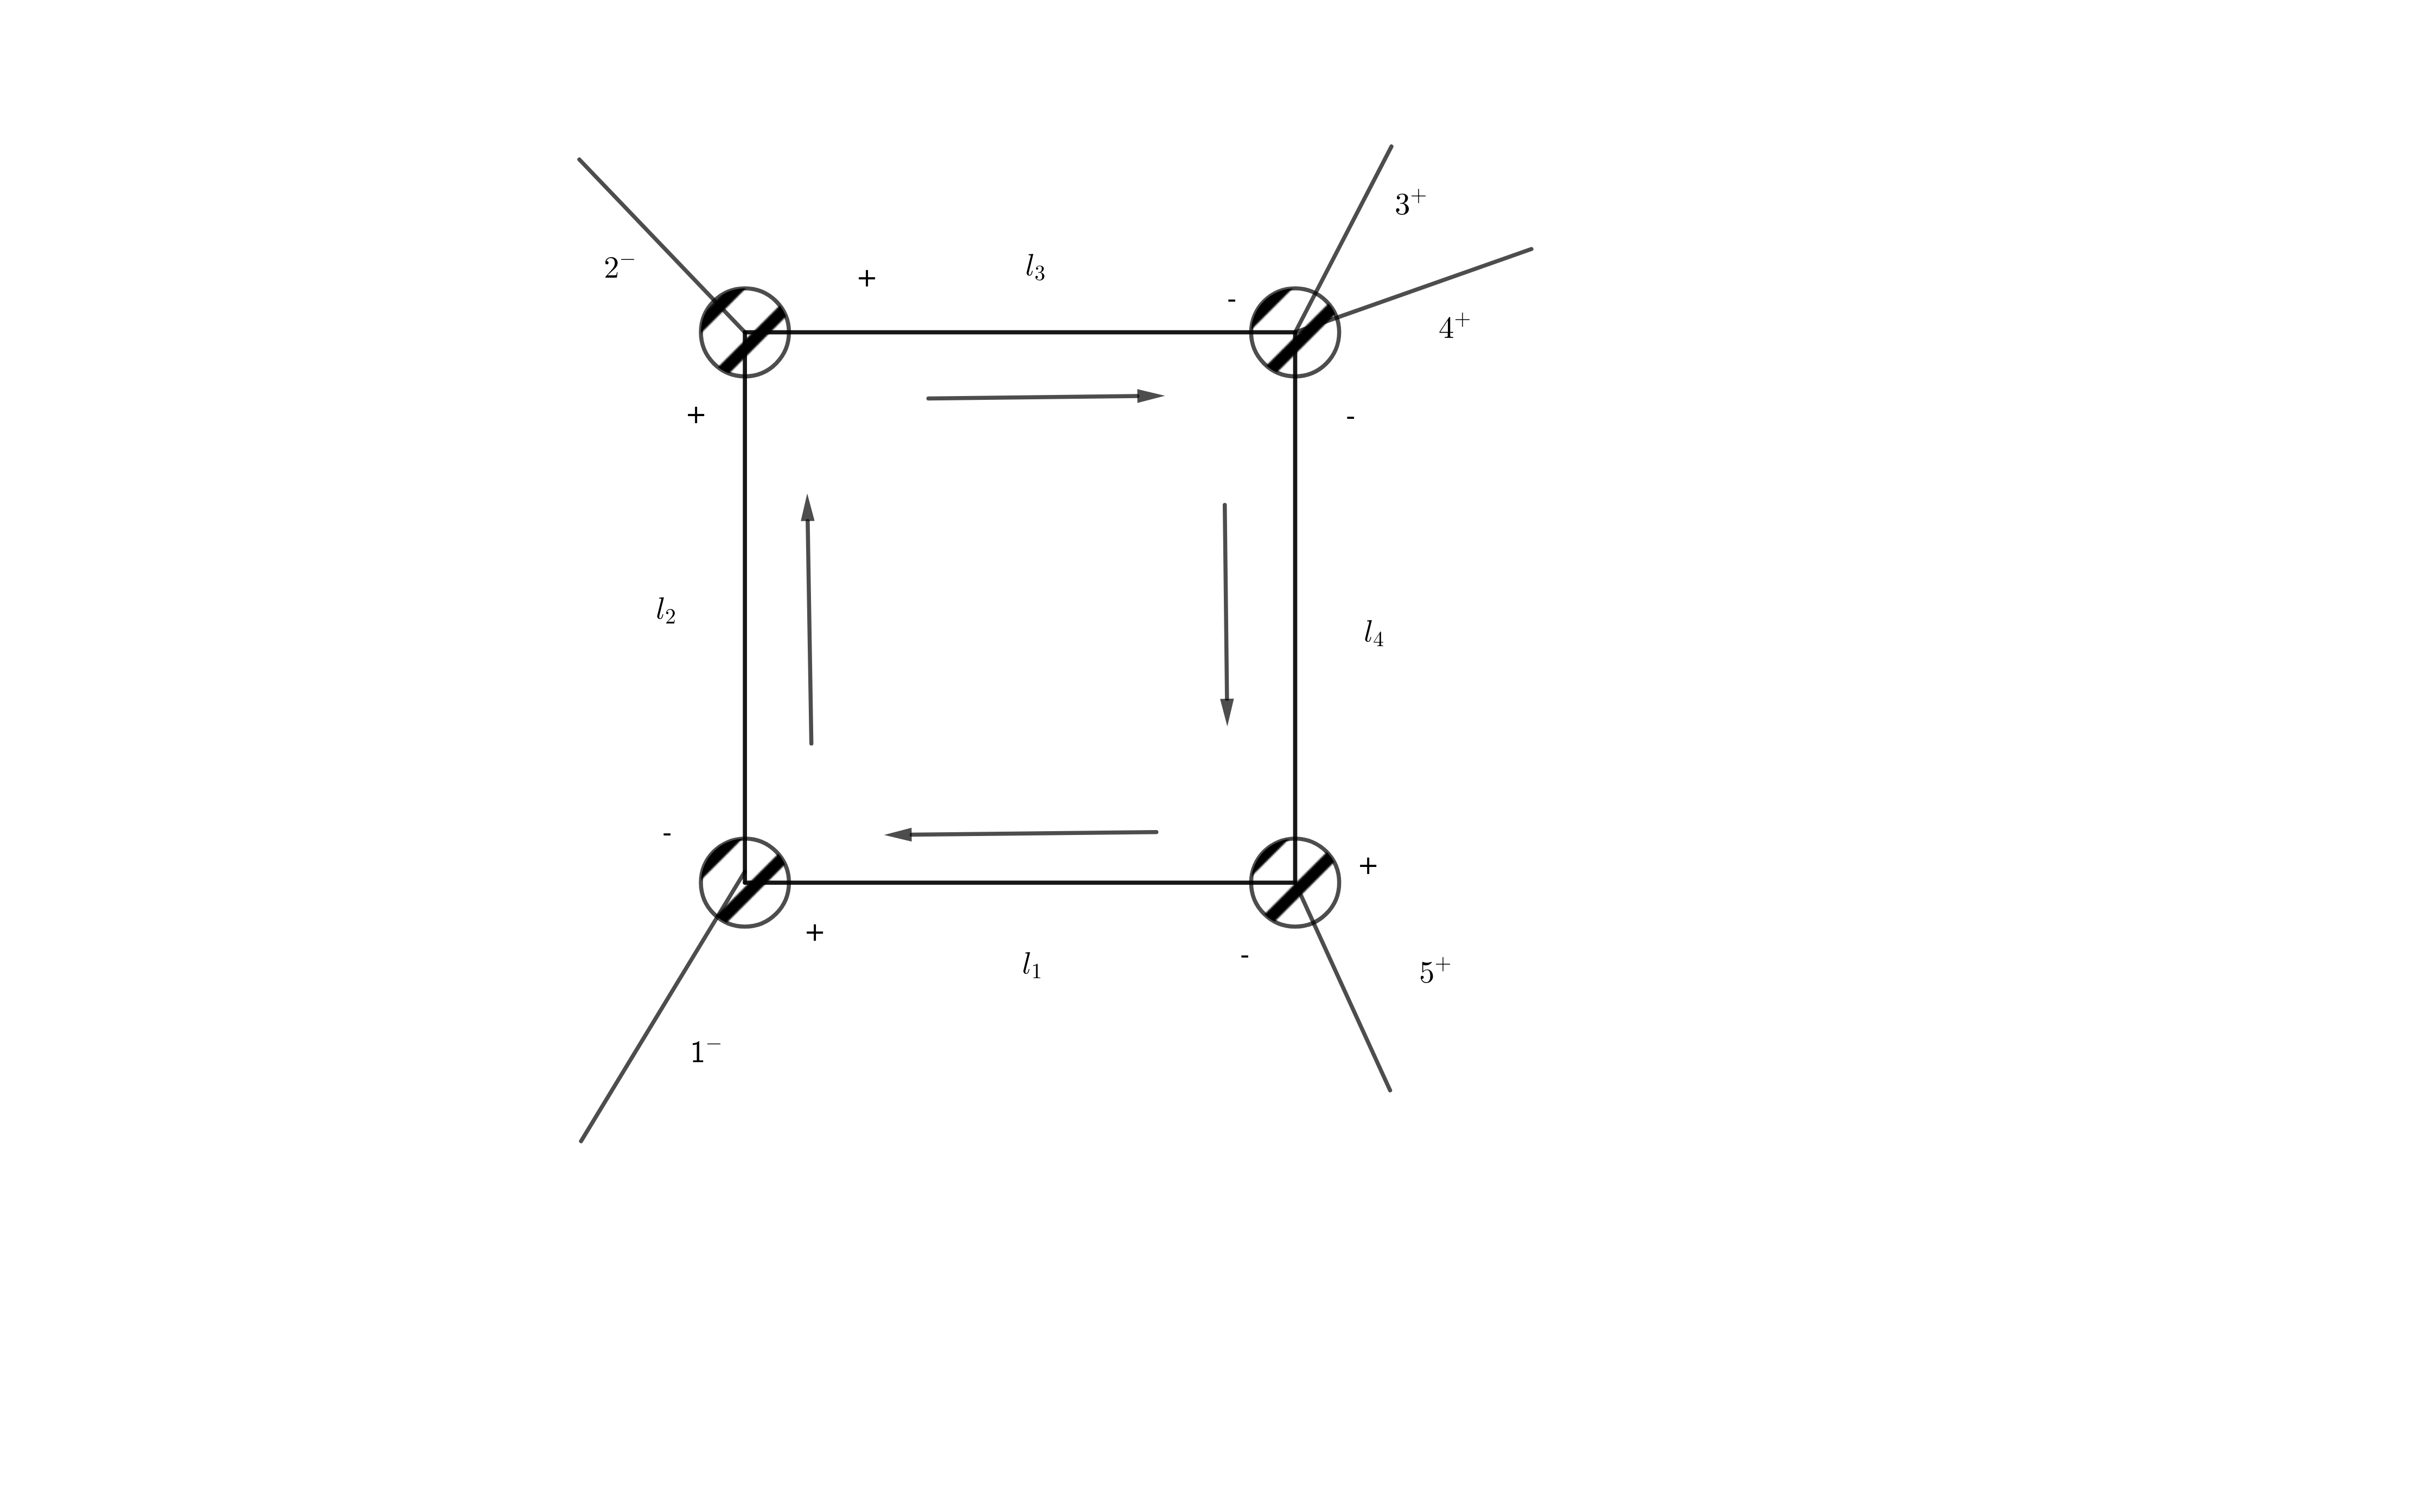
\includegraphics[width=\linewidth]{A5-10}
    \caption{A5-10}
  \label{A5-10}
\end{figure}
\fi
%
\paragraph{\ref{A5-10}}
\begin{equation*}
\begin{split}
c_{10} = &
\frac{1}{2}\frac{\langle 1l_2\rangle^3}{\langle l_2 l_1 \rangle\langle l_1 1 \rangle}
\frac{[l_2 l_3]^3}{[l_2 2 ][2 l_3]}
\frac{[34]^4}{[34][4 l_4][l_4 l_3][l_3 3]}
\frac{[l_4 5]^3}{[l_4 l_1][l_1 5]}
\\
= &
\frac{1}{2}\frac{\langle 12 \rangle^3[2l_3]^3[34]^3[l_4 5 ]^2}{\langle 51 \rangle[15][2l_3]^2\langle l_3 1\rangle [4 l_4][l_4 l_3][l_3 3]}
\end{split}
\end{equation*}
Set
\begin{equation*}
|l_3\rangle = \alpha |2\rangle \quad,\quad |l_3] = a|2] + b|5]
\quad,\quad
|l_4\rangle = \beta |5\rangle \quad,\quad |l_4] = c|2]+d|5]
\end{equation*}
Then
\begin{equation*}
\begin{split}
& (l_3 + K_{12})^2 = 0 \quad\Rightarrow\quad K_{12}^2 = - \alpha a [2|\slashed{K}_{12}|2\rangle - \alpha b [5|\slashed{K}_{12}|2\rangle
\\
& (l_3 - K_{34})^2 = 0 \quad\Rightarrow\quad K_{34}^2 = \alpha a [2|\slashed{K}_{34}|2\rangle + \alpha b [5|\slashed{K}_{34}|2\rangle
\end{split}
\end{equation*}
which leads to
\begin{equation*}
\alpha a = \frac{[5|\slashed{K}_{34}|5\rangle}{[25]\langle 52\rangle}
\\
\alpha b = \frac{[21]\langle 15\rangle}{[52]\langle 25\rangle}
\end{equation*}
On the other hand
\begin{equation*}
\begin{split}
& (l_4 - K_{45})^2 = 0 \quad\Rightarrow\quad
K_{15}^2 = \beta c[2|\slashed{K}_1|5\rangle + \beta d [5|\slashed{K}_1|5\rangle
\\
& (l_4 + K_{34})^2 = 0 \quad\Rightarrow\quad
K_{34}^2 = \beta c [2|\slashed{K}_1|5\rangle - \beta d [5|\slashed{K}_{34}|5\rangle
\end{split}
\end{equation*}
gives
\begin{equation*}
\beta c = - \frac{[51]\langle 12 \rangle}{[52]\langle 25 \rangle}
\quad,\quad
\beta d = - \frac{[2| \slashed{K}_{34}|2\rangle}{[5|\slashed{K}_2|5\rangle}
\end{equation*}
The coefficient $c_{10}$ is then given by
\begin{equation*}
c_{10} = 
\frac{1}{2}\frac{[21][34]^3[51]\langle 12\rangle^4 [52]^2 \langle 52\rangle[25]}{\big(-[42][51]\langle 12\rangle - [2|\slashed{K}_{34}|2\rangle [45]\big)
\big( K_{51}^2 K_{21}^2 - (2K_2\cdot K_{34})(2K_5\cdot K_{34})\big)
\big( [5|\slashed{K}_{34}|5\rangle [23] - [21]\langle 15\rangle [35]\big)
}
\end{equation*}
Using Schouten identity and the momentum conservation, we can rewrite the terms in the denominator in a more compact way
\begin{equation*}
\begin{split}
& -[42][51]\langle 12\rangle - [2|\slashed{K}_{34}|2\rangle [45] = 
-\langle 32\rangle[52][34]
\\
& K_{51}^2 K_{21}^2 - (2K_2\cdot K_{34})(2K_5\cdot K_{34}) = 
-s_{52}s_{34}
\\
& [5|\slashed{K}_{34}|5\rangle [23] - [21]\langle 15\rangle [35]
= -\langle 45\rangle[52][34]
\end{split}
\end{equation*}
As a result
\begin{equation*}
c_{10} = \frac{1}{2}s_{51}s_{12}A_5^{\textrm{MHV-tree}}[12345]
\end{equation*}
%
%
\iffalse
\begin{figure}
  \centering
    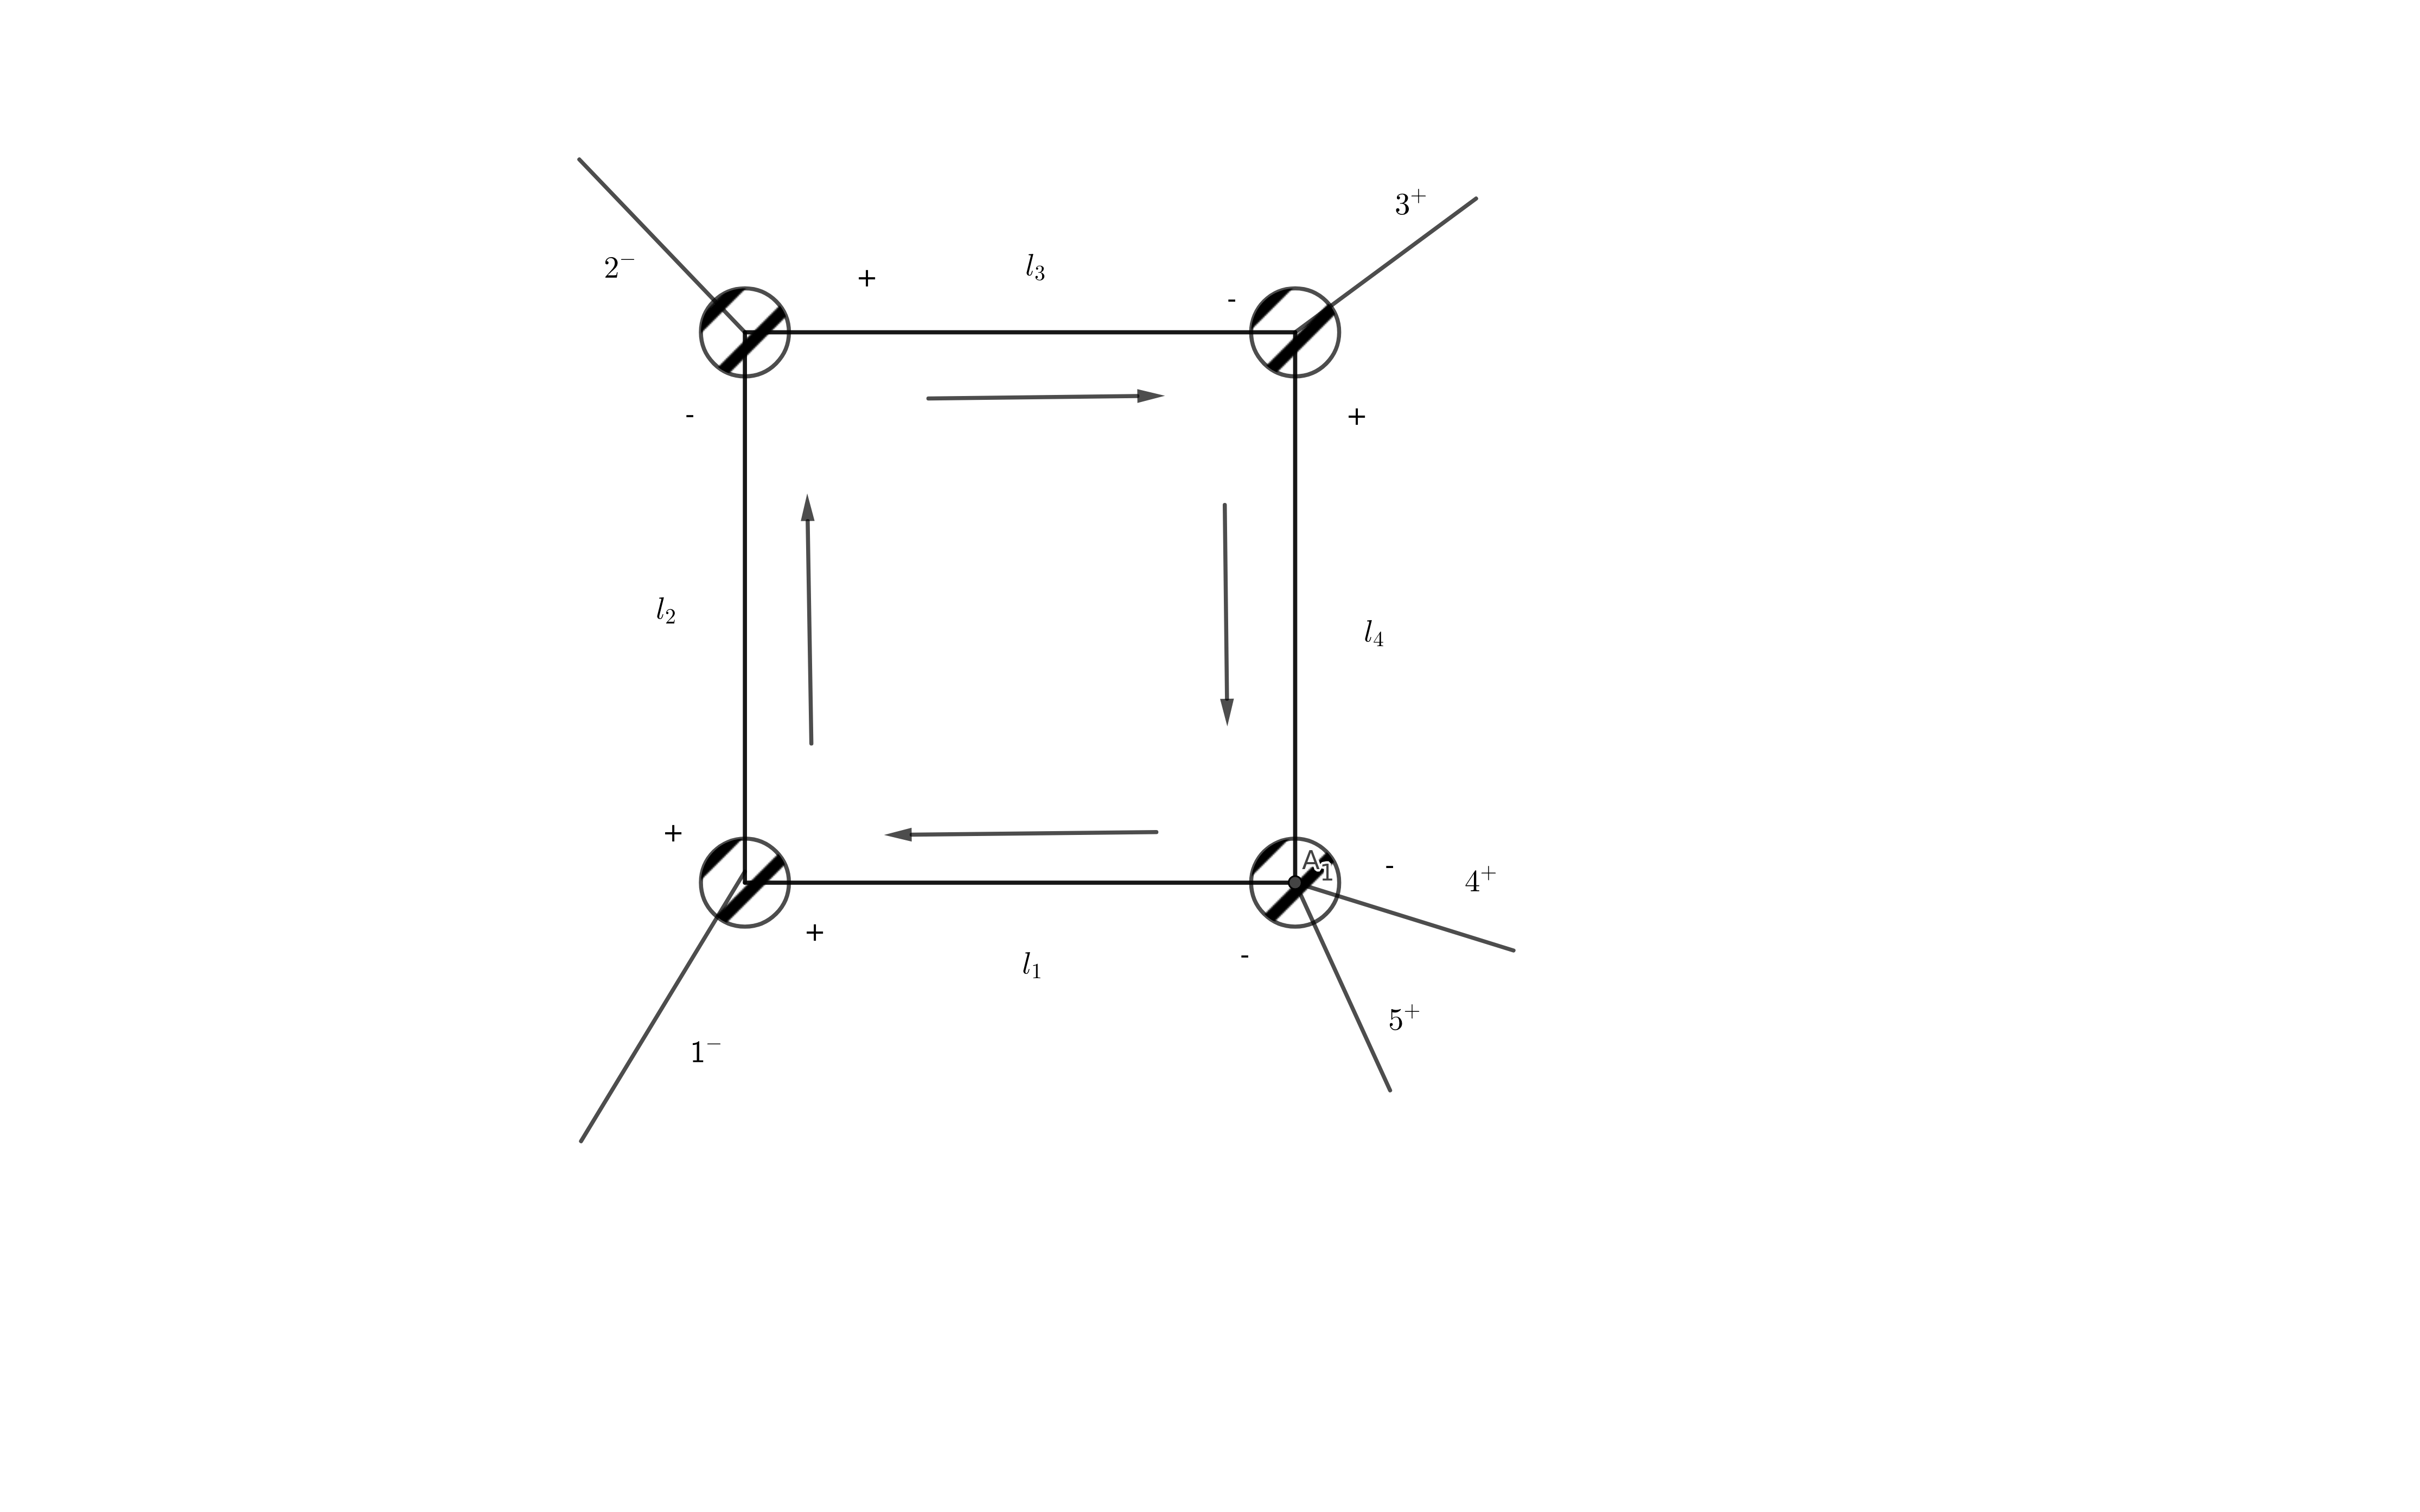
\includegraphics[width=\linewidth]{A5-11}
    \caption{A5-11}
  \label{A5-11}
\end{figure}
\fi
%
\paragraph{\ref{A5-11}}
\begin{equation*}
\begin{split}
c_{11} = &
\frac{1}{2}\frac{[l_1 l_2]^3}{[l_1 1][1l_2]}
\frac{\langle l_2 2 \rangle^3}{\langle 2 l_3 \rangle\langle l_3 l_2 \rangle}
\frac{[3l_4]^3}{[l_4 l_3][l_3 3]}
\frac{[45]^4}{[45][5l_1][l_1l_4][l_4 4]}
\\
= &
-\frac{1}{2}
\frac{[l_1 1]\langle 12 \rangle^3[3l_4]^2[45]^3}{[23]\langle l_1 2 \rangle\langle 23 \rangle[5l_1][l_1l_4][l_4 4]}
\end{split}
\end{equation*}
%
Set
\begin{equation*}
|l_1\rangle = \alpha| 1\rangle \quad,\quad
|l_1] = a|1] + b|3] \quad,\quad
|l_4\rangle = \beta|3\rangle 
| l_4] = c|1] + d|3]
\end{equation*}
Then
\begin{equation*}
\begin{split}
& (l_1- K_{12})^2 = 0 \quad\Rightarrow\quad K_{12}^2 = \alpha a [1|\slashed{K}_2|1\rangle + \alpha b [3|\slashed{K}_2|1\rangle
\\
& (l_1 + K_{45})^2 = 0 \quad\Rightarrow\quad
K_{45}^2 = -\alpha a [1|\slashed{K}_{45}|1\rangle - \alpha b [3|\slashed{K}_{45}|1\rangle
\end{split}
\end{equation*}
so
\begin{equation*}
\alpha a = \frac{[3|\slashed{K}_{12}|3\rangle}{[13]\langle 31\rangle}
\quad,\quad
\alpha b = \frac{[21]\langle 23\rangle}{[13]\langle 31\rangle}
\end{equation*}
On the other hand
\begin{equation*}
\begin{split}
& (l_4 + K_{23})^2 = 0 \quad\Rightarrow\quad K_{23}^2 = -\beta c[1|\slashed{K}_2|3\rangle - \beta d [3|\slashed{K}_2|3\rangle
\\
& (l_4 - K_{45})^2 = 0 \quad\Rightarrow\quad K_{45}^2 = \beta c [1|\slashed{K}_{45}|3\rangle + \beta d [3|\slashed{K}_{45}|3\rangle
\end{split}
\end{equation*}
Hence
\begin{equation*}
\beta c = \frac{[32]\langle 21\rangle}{[31]\langle 13\rangle}
\quad,\quad
\beta d = -\frac{[1|\slashed{K}_{23}|1\rangle}{[31]\langle 13\rangle}
\end{equation*}
and
\begin{equation*}
c_{11} = \frac{1}{2}\frac{[32][21][31]^4\langle 13\rangle\langle 12 \rangle^4 [45]^3}{\big( [3|\slashed{K}_{12}|3\rangle [51] + [21]\langle 23\rangle [53]\big)
\big( [32]\langle 21\rangle[14] - [1|\slashed{K}_{23}|1\rangle[34]\big)
\big( (2K_{12}\cdot K_3)(2K_{23}\cdot K_1) - K_{23}^2K_{21}^2\big)
}
\end{equation*}
Again, using Schouten identity and momentum conservation, we obtain the following equations which simplify the denominator
\begin{equation*}
\begin{split}
& [3|\slashed{K}_{12}|3\rangle [51] + [21]\langle 23\rangle [53] = -[31][54]\langle 43 \rangle 
\\
& -[13][45]\langle 51 \rangle
\\
&
(2K_{12}\cdot K_3)(2K_{23}\cdot K_1) - K_{23}^2K_{21}^2 = s_{45}s_{31}
\end{split}
\end{equation*}
At the end
\begin{equation*}
c_{11} = \frac{1}{2}s_{12}s_{23}A_5^{\textrm{MHV-tree}}[12345]
\end{equation*}
%
%
\iffalse
\begin{figure}
  \centering
    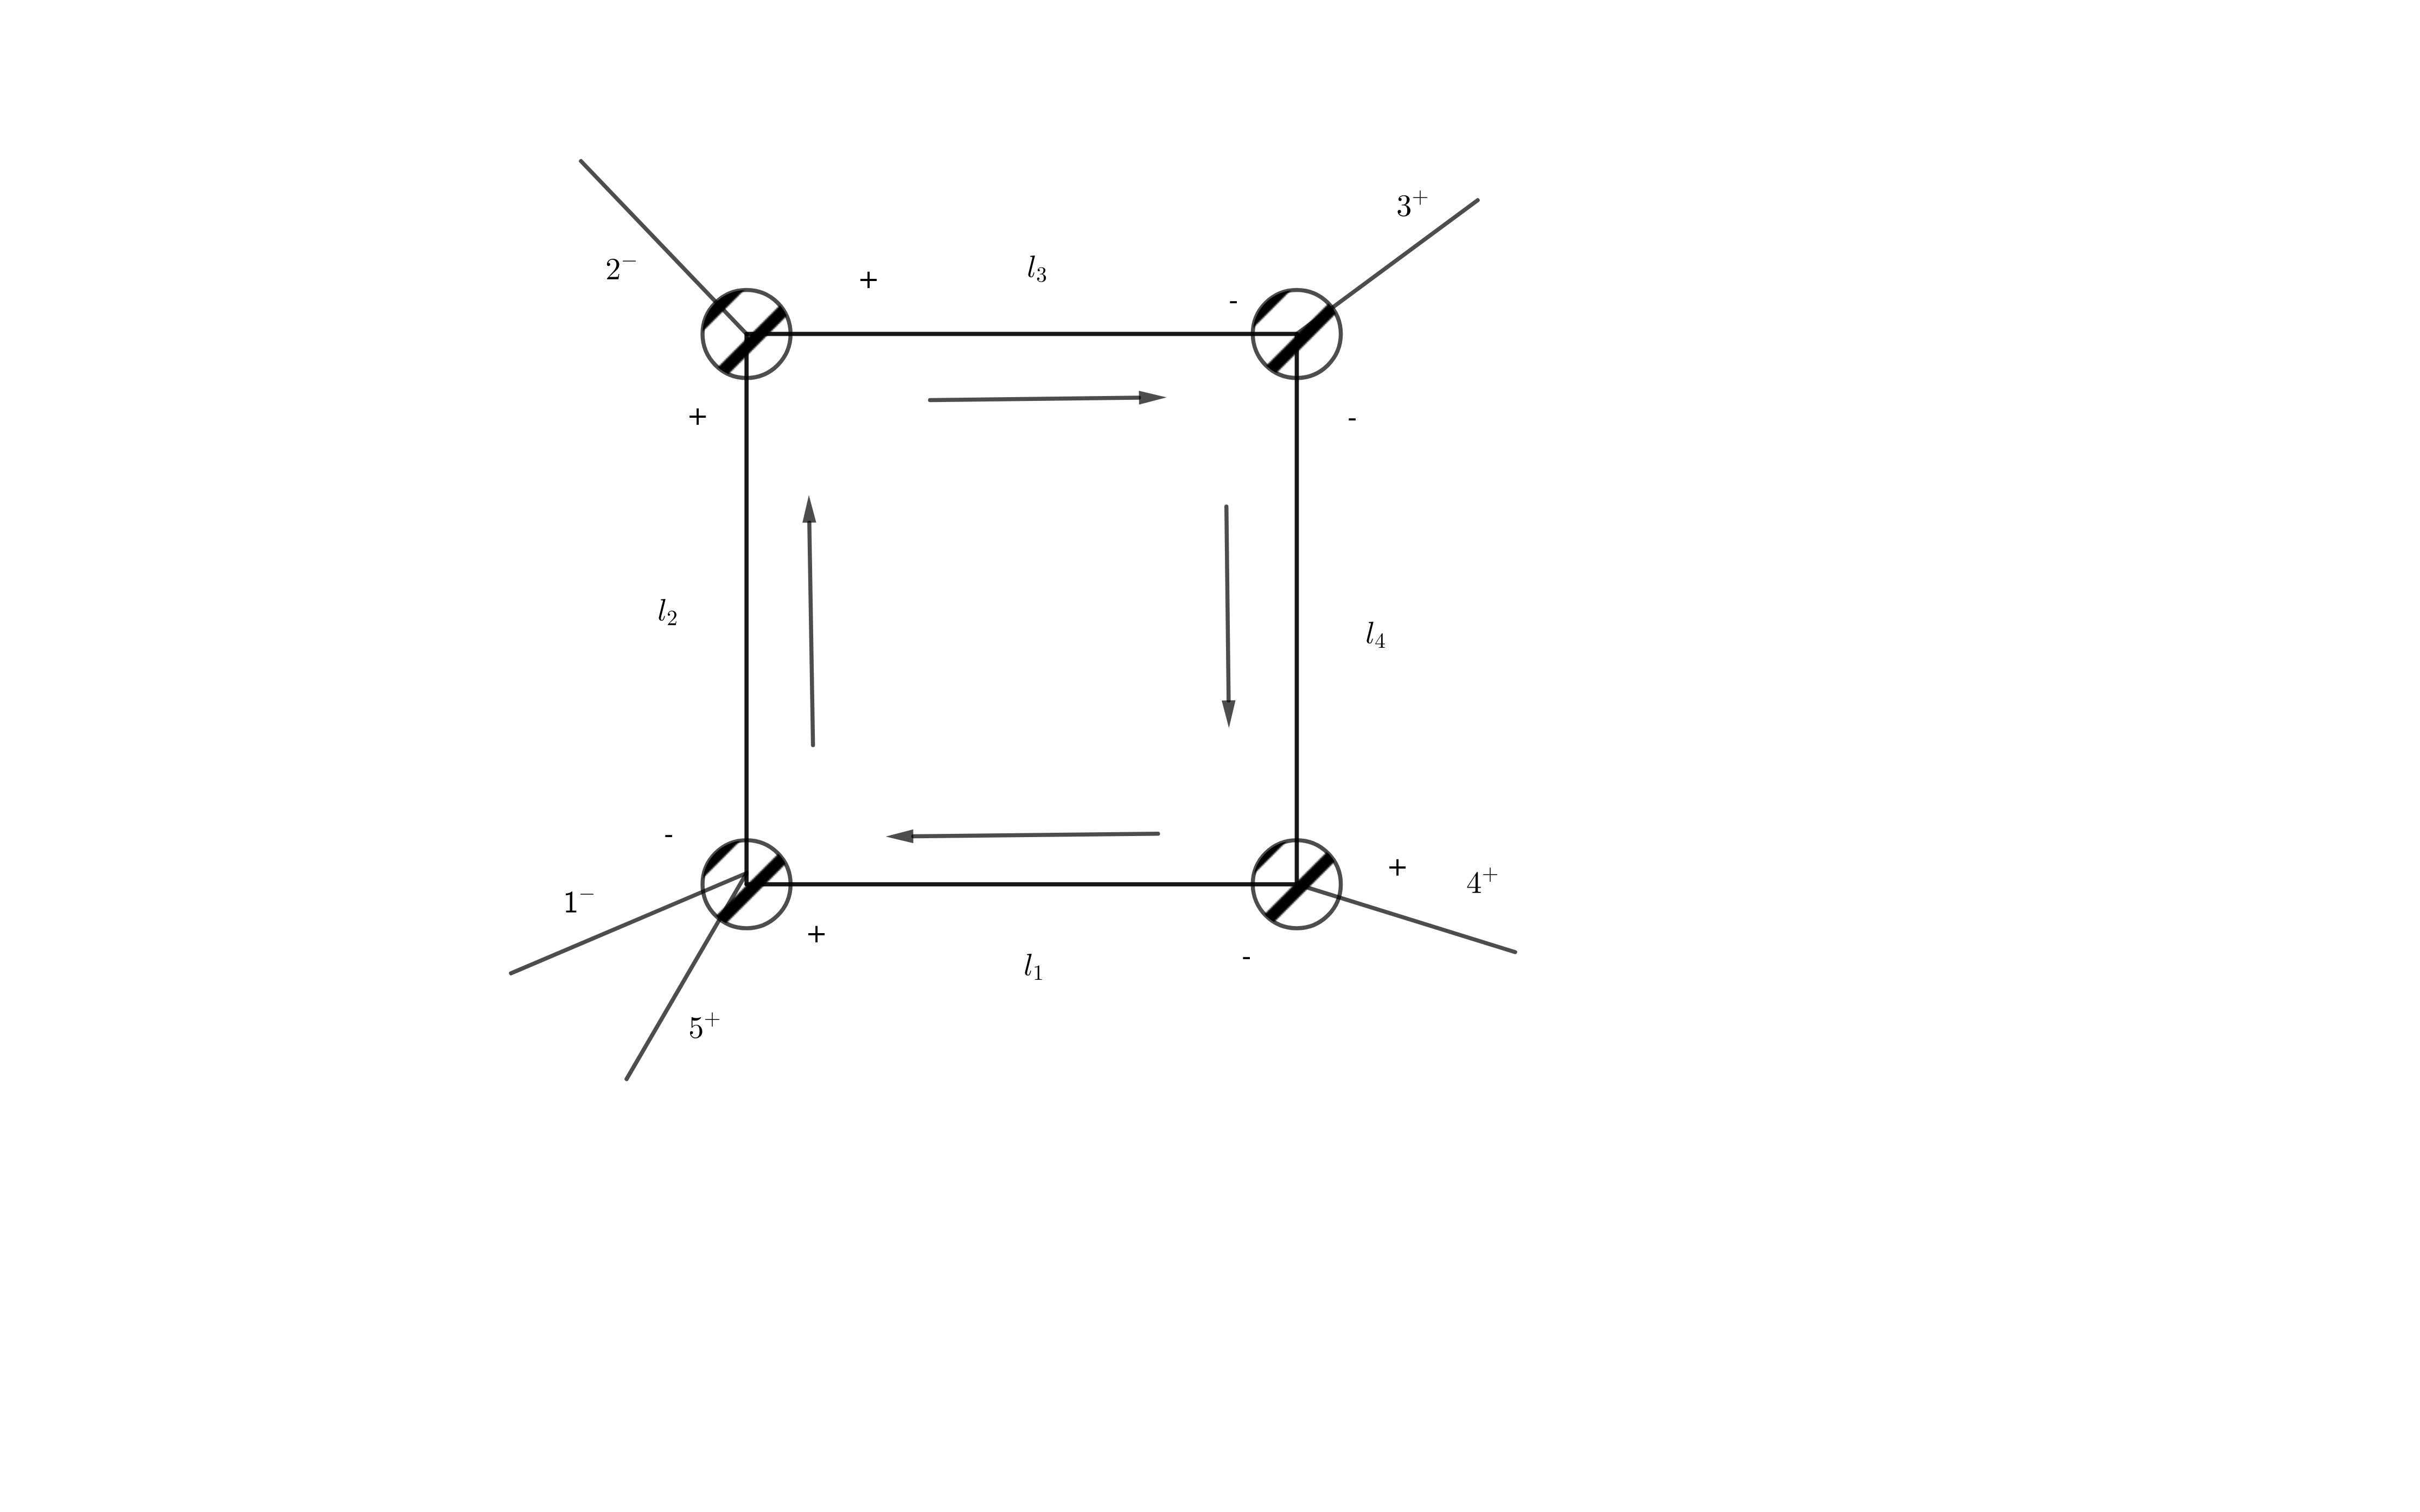
\includegraphics[width=\linewidth]{A5-16}
    \caption{A5-16}
  \label{A5-16}
\end{figure}
\fi
%
%
\paragraph{\ref{A5-16}}
\begin{equation*}
\begin{split}
c_{16} = & \frac{1}{2}
\frac{\langle l_2 1 \rangle^4}{\langle l_2 1 \rangle\langle 15 \rangle\langle 5 l_1 \rangle\langle l_1 l_2\rangle}
\frac{[l_2 l_3]^3}{[l_3 2 ][2 l_2]}
\frac{\langle l_3 l_4\rangle^3}{\langle l_3 3\rangle\langle 3 l_4\rangle}
\frac{[l_4 4 ]^3}{[4l_1][l_1l_4]}
\\
= & 
-\frac{1}{2}\frac{\langle l_2 1\rangle^3[l_2 2 ]\langle 23 \rangle^3[34]^3}{\langle 15 \rangle[4l_4]\langle l_4 l_2\rangle\langle 3l_2\rangle \langle 3 l_4\rangle\langle 54\rangle[4l_4]}
\end{split}
\end{equation*}
Set
\begin{equation*}
|l_2\rangle = \alpha|2\rangle \quad,\quad
|l_2] = a|2] + b|4] \quad,\quad
|l_4\rangle = \beta |4\rangle \quad,\quad
|l_4] = \gamma|3]
\end{equation*}
Then
\begin{equation*}
\begin{split}
& (l_2 - K_{23})^2 = 0 \quad\Rightarrow\quad K_{23}^2 = \alpha a [2|\slashed{K}_3|2\rangle + \alpha b [4|\slashed{K}_{23}|2\langle
\\
& (l_2 + K_{15})^2 = 0 \quad\Rightarrow\quad K_{15}^2 = -\alpha a [2|\slashed{K}_{15}|2\rangle - \alpha b [4|\slashed{K}_{15}|2\rangle
\end{split}
\end{equation*}
\begin{equation*}
\begin{split}
& \alpha a = \frac{[4|\slashed{K}_{23}|4\rangle}{[24]\langle 42\rangle}
\\
& \alpha b = \frac{[32]\langle 34\rangle}{[24]\langle 42\rangle}
\end{split}
\end{equation*}
On the other hand
\begin{equation*}
(l_4 + K_{23})^2 = 0 \quad,\quad \beta\gamma = \frac{\langle 32\rangle}{\langle 24\rangle}
\end{equation*}
Thus
\begin{equation*}
c_{16}= \frac{1}{2}\frac{\langle 21\rangle^3[34][32]}{\langle 15\rangle\langle 54\rangle} = \frac{1}{2}s_{23}s_{34}A_5^{\textrm{MHV-tree}}[12345]
\end{equation*}
%
%
%
The last question: how about the other remaining possible intermediate species such as fermions and scalars?
These configurations should of course also be taken into account.
One might think of using the supersymmetry Ward identities~\cref{super_wi} to compute them. 
In fact, the total contribution of these configurations vanishes.
This can be done by a rather trivial analysis of the above helicity configurations.
Let us recall the action of a $\mathcal{N} = 4$ super Yang-Mills theory (cf. \eg Eq.(4.19) of~\cite{Elvang:2013cua})
\begin{equation*}
S = \int \dd^4 x\tr\Big(
-\frac{1}{4}F_{\mu\nu}F^{\mu\nu} - \frac{1}{2}\big(D\Phi_I)^2 + \frac{i}{2}\bar{\Psi}\slashed{D}\Psi + \frac{g}{2}\bar{Psi}\Gamma^I \big[\Phi_I, \Psi\big] + \frac{g^2}{4}\big[\Phi_I, \Phi_J\big]^2\Big) 
\end{equation*}
where $\Phi_I$'s are six real scalar field, fermions are represented by the ten-dimensional Majorana-Weyl spinor $\Psi$, $D$ is the usual covariant derivative and $F_{\mu\nu}$ represents the gluon field strength.
In the context of~\cref{super_wi}, we will consider complex scalar fields made of the real scalar ones instead. 
Without giving the action written with complex scalar fields, we just state that, at tree-level, complex scalars and fermions always come up in pair with their conjugate fields when coupled with gluons. 
Recall that our convention is to take all the particles outgoing in an amplitude.
All of the non-vanishing helicity configurations given above involve at least one tree-level amplitude with the same helicity for the cut propagator in the product~\cref{box_coeff}.
Since it is impossible to have such a tree-level contribution with other intermediate species than gluons, the corresponding species configurations vanish.
\\\\
In consequence, the five-point MHV all-gluon amplitude $A_5^{\mathrm{1-loop}}[--+++]$ is given by
\begin{equation}
A_5^{\mathrm{1-loop}}[--+++] = c_1 I_{1} + c_8 I_8 + c_{10}I_{10} + c_{11}I_{11} + c_{16}I_{16}
\end{equation}
where the $I_{k}$'s are the corresponding box integral for each configuration.
This result is in agreement with~\cite{Bern:1994zx}.














